
%Class
	\documentclass[a4paper,12pt]{article}

%Packages
	\usepackage{amsmath}					% Standard maths
	\usepackage{amssymb}					% Standard maths
	\usepackage{amsthm}						% Standard maths
	\usepackage{thmtools, thm-restate}% Theorem styles
	\usepackage{mathtools}
	\usepackage[newzealand]{babel}% Date/time in British format (yes, I know it says NZ)
	\usepackage{datetime}					% Date/time
	\usepackage{multirow}					% For stacked subscripts
	\usepackage{xcolor}						% For colour!
	\usepackage[normalem]{ulem}		% For strikeout
	\usepackage{isomath}
	\usepackage{fancyhdr}					% For the headers
	\usepackage{mfirstuc}					% For the headers
	\usepackage[hmargin=1in,top=0.8in,bottom=1in]{geometry} % Page margins more reasonable
	\usepackage{graphicx}					% For including graphics
	%\usepackage{float}						% For something
	\usepackage{enumitem}					% For numbering tweaks
	\usepackage{pgfplots}
	\usepackage[margin=15pt,font={footnotesize},labelfont=bf,format=hang]{caption}
\usepackage[margin=15pt,font={footnotesize},labelfont=bf,format=hang]{subcaption}
	\usepackage{url}
	\usepackage[hidelinks]{hyperref}	% For hyperlinks
	\usepackage{breakurl}
	\usepackage{cleveref}
	\usepackage[scaled=.92]{helvet}

%MATHEMATICAL SHORTCUTS
%Two and three-part definitions
	\newcommand{\twopartdef}[4]
	{	\left\{
			\begin{array}{ll}
				#1 & \mbox{if } #2 \\
				#3 & \mbox{if } #4
			\end{array}
		\right.}
%	\newcommand{\threepartdef}[6]
%	{	\left\{
%			\begin{array}{ll}
%				#1 & \mbox{if } #2 \\
%				#3 & \mbox{if } #4 \\
%				#5 & \mbox{if } #6
%			\end{array}
%		\right.}
%Blackboard bold	
	\newcommand{\N}{{\mathbb N}} 
	\newcommand{\R}{{\mathbb R}} 
	\newcommand{\C}{{\mathbb C}} 
	%Curly letters
%	\newcommand{\E}{{\mathcal E}}	
%	\newcommand{\F}{{\mathcal F}} 
%	\newcommand{\Null}{{\mathcal N}} 
%	\newcommand{\R}{\mathcal{R}} 
%	\newcommand{\Z}{\mathcal{Z}} 
%Uprights
	\newcommand{\D}{{\mathrm D}}
	\renewcommand{\d}{{\mathrm d}}
%Easy Greeks
%	\def\a{\alpha}
%	\def\g{\gamma}
%	\newcommand{\e}{{\varepsilon}}
%	\newcommand{\la}{{\lambda}}  
%	\newcommand{\om}{{\Omega}}
	\renewcommand{\epsilon}{\varepsilon}
	
%Vector operators
	\def \p {\partial}
	\newcommand{\del}{{\nabla}}
	\newcommand{\grad}{{\nabla}}
    \newcommand{\vdel}{\boldsymbol{\nabla}}
    \newcommand{\vgrad}{\boldsymbol{\nabla}}
    \newcommand{\vnabla}{\boldsymbol{\nabla}}
	\newcommand{\cross}{{\times}}
	\newcommand{\Lap}{{\nabla^2}} 
%Arrows
%	\newcommand{\goesto}[1]{\xrightarrow[#1]{}}
%hats
%	\newcommand{\nhat}{\widehat{\v{n}}}
%	\newcommand{\shat}{\widehat{\v{s}}}
	\renewcommand{\hat}{\widehat}
%Note to self
%	\newcommand{\note}[1]{[\textbf{\textsl{\MakeUppercase{#1}}}]}
	
%Stress tensor
%	\newcommand{\T}{\vg{\sigma}}

% Vectors, quaternions etc.
\renewcommand{\v}[1]{\mathbfit{#1}}      % Generic vector
\newcommand{\vc}[1]{\bm{\mathcal{#1}}}      % vector mathcal
\newcommand{\uv}[1]{\widehat{\mathbfit{#1}}}      % Generic unit vector
\newcommand{\q}[1]{\mathsfbfit{#1}}        % Generic quaternion
\renewcommand{\t}[1]{\mathsfbfit{#1}}	 % Generic tensor
\newcommand{\m}[1]{\mathsfbfit{#1}}	 % Generic matrix
\newcommand{\vu}[1]{\mathbf{#1}}         % Upright vector (for zero vector)
\newcommand{\qu}[1]{\mathbf{#1}}       % Upright quaternion (for zero quaternion)
\newcommand{\tu}[1]{\bm{\mathsf{#1}}}	 % Upright tensor (for zero tensor)

%Real and imaginary
\renewcommand{\Re}{\operatorname{Re}}
\renewcommand{\Im}{\operatorname{Im}}
	
%Non-dim numbers
%	\renewcommand{\Re}{\operatorname{Re}}
%	\newcommand{\Bi}{\operatorname{Bi}}
%	\newcommand{\Fo}{\operatorname{Fo}}
	
%Misc
\DeclareMathSymbol{\Delta}{\mathalpha}{operators}{1} % Keeps Delta upright
\DeclareMathSymbol{\Gamma}{\mathalpha}{operators}{0} % Keeps Gamma upright
	\newcommand{\cosec}{\operatorname{cosec}}
	\newcommand{\cosech}{\operatorname{cosech}}
	\newcommand{\sech}{\operatorname{sech}}
	\newcommand{\tr}{\operatorname{tr}}
	\newcommand{\erf}{\operatorname{erf}}
	\newcommand{\order}{\mathcal{O}}
%	\newcommand{\V}{\mathcal{V}} % 	CurlyV = (Bi V) / (1 + Bi)

% Differentiating 
\newcommand{\fd}[2]{\mathchoice{\frac{\d #1}{\d #2}}{\d #1/\d #2}{\d #1/\d #2}{\d #1/\d #2}}
\newcommand{\fdd}[2]{\mathchoice{\frac{\d^2 #1}{\d #2^2}}{\d^2 #1/\d #2^2}{\d^2 #1/\d #2^2}{\d^2 #1/\d #2^2}}
\newcommand{\fddd}[2]{\mathchoice{\frac{\d^3 #1}{\d #2^3}}{\d^3 #1/\d #2^3}{\d^3 #1/\d #2^3}{\d^3 #1/\d #2^3}}
\newcommand{\fdddd}[2]{\mathchoice{\frac{\d^4 #1}{\d #2^4}}{\d^4 #1/\d #2^4}{\d^4 #1/\d #2^4}{\d^4 #1/\d #2^4}}
\newcommand{\fdn}[3]{\mathchoice{\frac{\d^{#1} #2}{\d #3^{#1}}}{\d^{#1} #2/\d #3^{#1}}{\d^{#1} #2/\d #3^{#1}}{\d^{#1} #2/\d #3^{#1}}}
\newcommand{\pd}[2]{\mathchoice{\frac{\p #1}{\p #2}}{\p #1/\p #2}{\p #1/\p #2}{\p #1/\p #2}}
\newcommand{\pdd}[2]{\mathchoice{\frac{\p^2 #1}{\p #2^2}}{\p^2 #1/\p #2^2}{\p^2 #1/\p #2^2}{\p^2 #1/\p #2^2}}
\newcommand{\pddmixed}[3]{\frac{\p^2 #1}{\p #2 \p #3}}
\newcommand{\pddd}[2]{\frac{\p^3 #1}{\p #2^3}}
\newcommand{\pdn}[3]{\mathchoice{\frac{\p^{#1} #2}{\p #3^{#1}}}{\p^{#1} #2/\p #3^{#1}}{\p^{#1} #2/\p #3^{#1}}{\p^{#1} #2/\p #3^{#1}}}
	
	% Misc
\newcommand{\e}{\mathrm{e}}
\renewcommand{\i}{\mathrm{i}}
\newcommand{\dx}{\,\mathrm{d}x}
\newcommand{\dy}{\,\mathrm{d}y}
\renewcommand{\epsilon}{\varepsilon}
\renewcommand{\Re}{\operatorname{Re}}
\newcommand{\Four}{\mathcal{F}}

\newcommand{\mat}[4]{\begin{pmatrix}#1 & #2 \\ #3 & #4 \end{pmatrix}}

	%Column vectors
	\makeatletter
\newcommand\rcvector[2][\\]{\ensuremath{%
  \global\def\rc@delim{#1}%
    \negthinspace\begin{pmatrix}
      \rc@vector #2,\relax\noexpand\@eolst%
    \end{pmatrix}}}
\def\rc@vector #1,#2\@eolst{%
  \ifx\relax#2\relax
    #1
  \else
    #1\rc@delim
    \rc@vector #2\@eolst%
  \fi}
\makeatother

\newcommand{\colvec}{\rcvector}
\newcommand{\rowvec}{\rcvector}
\renewcommand{\binom}{\rcvector}
	
	%Colours
%	\newcommand{\orange}[1]{{\color{orange} #1 }}
%	\newcommand{\blue}[1]{{\color{blue} #1 }}

%Theorem styles
%	\declaretheoremstyle[headpunct={\:\:\:}, shaded={bgcolor={rgb}{0.9,0.9,0.9}, margin=5pt}]{problem}
%	\declaretheoremstyle[headpunct={\:\:\:}, shaded={rulecolor=black, rulewidth=0.4pt, bgcolor={rgb}{1,1,1}, margin=5pt}]{definition}
%	\declaretheoremstyle[headpunct={\:\:\:}, spaceabove=15pt, notefont=\bf, notebraces={(}{)}]{theorem}
%	\declaretheoremstyle[headpunct={\:\:\:}, numbered=no, spaceabove=15pt, qed={\checkmark}]{solution}
%	
%	\declaretheorem[style=definition,numberwithin=section]{definition}
%	\declaretheorem[numberlike=definition, style=theorem]{theorem}
%	\declaretheorem[numberlike=definition, style=theorem]{lemma}
%	\declaretheorem[numberlike=definition,style=problem]{problem}
%	\declaretheorem[numberlike=definition, style=theorem]{proposition}
%	\declaretheorem[numberlike=definition, style=theorem]{corollary}
%	\declaretheorem[numberlike=definition, style=theorem]{remark}
%	\declaretheorem[numberlike=definition, style=theorem]{example}
%	\declaretheorem[numberlike=definition, style=theorem]{notation}
%	\declaretheorem[style=solution]{solution}

%Depth of display breaks to allow	
	\allowdisplaybreaks[1]

%How deep do we want the Table of Contents to go?	
%	\setcounter{tocdepth}{1}

%Sections
\makeatletter
\renewcommand{\section}{\@startsection
{section}%                   % the name
{1}%                         % the level
{0mm}%                       % the indent
{-\baselineskip}%            % the before skip
{0.5\baselineskip}%          % the after skip
{\normalfont\bfseries}} % the style
\makeatother

% Wavy underline
\makeatletter
\font\sixly=lasyb10 scaled 1200
\def\tinners{\bgroup \markoverwith{\lower8.5\p@\hbox{\sixly \char58}}\ULon}
\makeatother
\newcommand{\answer}[1]{\tinners{\; #1 \;}}

%Setting the footnotes to use *,**,+ etc rather than 1,2,3	
\renewcommand{\thefootnote}{\fnsymbol{footnote}}

%Italic quote environment
%\newenvironment{quoteitalic}{\begin{quote}\itshape}{\end{quote}}

%Heading
\newcommand{\heading}[1]{
\setlength{\parindent}{0pt}
\textbf{MATH3171 (Mathematical Biology III)}

\textbf{YEAR 2025--26}%, MICHAELMAS TERM}
\setlength{\parskip}{3ex}

\textbf{\MakeUppercase{#1}}
%
\setlength{\parskip}{2ex}

}

%========================================================================================================================
%DOCUMENT BEGINS HERE!

\begin{document} 
%
\heading{Michaelmas revision class}
This sheet contains what was written on the board in the revision class on Monday 27 April 2026.

\section{General exam advice}
\begin{enumerate}[label=(\alph*)]
	\item Format: 
		\begin{itemize}
			\item Section A: Q1--4. 10 marks each.
			\item Section B: Q5--8. 15 marks each.
			\item No choice.
		\end{itemize}
	\item Within each sections, questions do not increase in difficulty.
	\item Think about order (read it all first).
	\item Think about timing -- how long to give to each question.
	\item Read the whole question. Maybe something at the end will tell you a hint or an assumption you can use.
	\item Lost? Can you do part (b) even if you can't do part (a)? This might require having to write down an assumption but that's OK.
	\item Move on! Use the mark distribution for time guidance.
	\item Use lots of paper! (Ask for more!)
	\begin{enumerate}[label=(\roman*)]
		\item no rough paper
		\item I will mark everything unless you cross it out
		\item new question, new page
		\item I want to give you marks, so make it easy for me! Write neatly!
	\end{enumerate}
\end{enumerate}	

\section{Math Bio exam advice}
\begin{enumerate}[label=(\alph*)]
	\item Do last year's paper and the practice paper already! (Don't save it.)
	\item Use bullet points.
	\item Draw pictures.
\end{enumerate}

\section{Rough course outline}
\begin{enumerate}[label=(\alph*)]
	\item 1D population models (time-dependent only)
	\begin{enumerate}[label=(\roman*)]
		\item equilibria (feasible/permissible)
		\item stability (drawing the phase space graph of $\fd{x}{t}$ against $x$ is nearly always the best way to determine stability in 1D)
		\item interpretation (drawing a picture is again the best method)
	\end{enumerate}
	\item 1D \& 2D population models
	\begin{enumerate}[label=(\roman*)]
		\item nondimensionalisation
		\item linear stability analysis formally (with $\varepsilon$)
		\item bifurcations (changes in the number or behaviour of equilibria): drawing bifurcation diagrams for 1D models and interpreting them
	\end{enumerate}
	\item 2D population models
	\begin{enumerate}[label=(\roman*)]
		\item linear stability analysis shortcuts (just writing down $\m{J}$, det/tr rules)
		\item phase portraits (draw and interpret)
	\end{enumerate}
	\item 3D population models
	\begin{enumerate}[label=(\roman*)]
		\item e.g.\ SIR
		\item reduction to 2D
	\end{enumerate}
	\item (advection--)diffusion
	\begin{enumerate}[label=(\roman*)]
		\item derivations
		\item separation of variables (bounded domain)
		\item Fourier transforms and Green's functions (unbounded domain)
		%\item similarity solutions (finite diffusion)
	\end{enumerate}
	\item travelling waves
	\begin{enumerate}[label=(\roman*)]
		\item existence (between which equilibria?)
		\item stability (indicating permissible wavespeeds)
	\end{enumerate}
	\item PDE stability (the start)
\end{enumerate}
%
\section{How an exam question is written}
\begin{itemize}
	\item The little bolt-on (e.g.\ interpret, non-dimensionalise, consider a simpler version)
	\item The meat
	\item Something that tests understanding
\end{itemize}
%
\section{Bifurcations}
You need to be able to go between
\[ \text{single-species model} \longleftrightarrow \text{bifurcation diagram}.\]
For example,
\[\fd{x}{t} = x-k\]
has equilibrium $x_0=k$. Is it stable or unstable? 

Drawing the phase portrait shows that $k$ is unstable.

So drawing the bifurcation diagram of $x_0$ again $k$, you get a dotted line of slope 1 which passes through the origin.

You should practice this for single-species (aka 1D) models that we've seen.

If you saw a bifurcation diagram, can you write down what $\fd{x}{t}$ should be?

\section{Nondimensionalisation}
e.g.\ \textbf{Exam 2022 Q2}:

Convert
\[ \pd{u}{t} = D \pdd{u}{x} + ru\left(1-\frac{u}{K}\right), \quad x \in [0,L] \]
into, after hats have been removed,
\[ \pd{u}{t} = \pdd{u}{x} + \alpha u(1-u), \quad x \in [0,1].\]

Normal procedure:
\[ u = U \hat{u}, \quad x = X\hat{x}, \quad t = T\hat{t},\]
which includes substituting in the interval definition:
\begin{align*}
	\frac{U}{T} \pdd{\hat{u}}{\hat{t}} &= \frac{DU}{X^2}\pdd{\hat{u}}{\hat{x}}+rU\hat{u}\left(1-\frac{U\hat{u}}{K}\right), \quad X \hat{x} \in [0,L]\\
	\implies \pdd{\hat{u}}{\hat{t}} &= \frac{DT}{X^2}\pdd{\hat{u}}{\hat{x}}+rT\hat{u}\left(1-\frac{U\hat{u}}{K}\right), \quad \hat{x} \in \left[0,\frac{L}{X}\right]
\end{align*}
Starting with the interval definition, we get $X=L$. The diffusion term gives us $T = L^2/D$. Therefore $\alpha = rT = rL^2/D$.

If we have a boundary condition, e.g.
\[u(L,t) = \beta,\]
Think about what this means. It means
\begin{align*}
	u = \beta \; & \text{when} \; x=L \; \text{and} \; \forall t \\
	\implies U\hat{u} = \beta \; & \text{when} \; X\hat{x}=L \; \text{and} \; \forall T\hat{t} \\
	\implies \hat{u} = \frac{\beta}{U} \; & \text{when} \; \hat{x}=\frac{L}{X} \; \text{and} \; \forall \hat{t},
\end{align*}
i.e.
\[\hat{u}\left(\frac{L}{X},\hat{t}\right) = \frac{\beta}{U}.\]

\section{Phase portraits}
e.g.\ \textbf{Exam 2022 Q8.5}:

System is
\begin{align*}
	\fd{S}{t} &= \alpha(N-S-I)-\beta IS - \nu S,\\
	\fd{I}{t} &= \beta IS - \gamma I.
\end{align*}
It has nullclines
\begin{align*}
	0 &= \alpha(N-S-I)-\beta IS - \nu S &&\implies I = \frac{\alpha N-(\alpha+\nu)S}{\alpha+\beta S},\\
	0 &= I(\beta S - \gamma) && \implies I = 0, \, S = \frac\gamma\beta.\end{align*}

Remember that nullclines can be curves, not just straight lines.
\begin{center}
	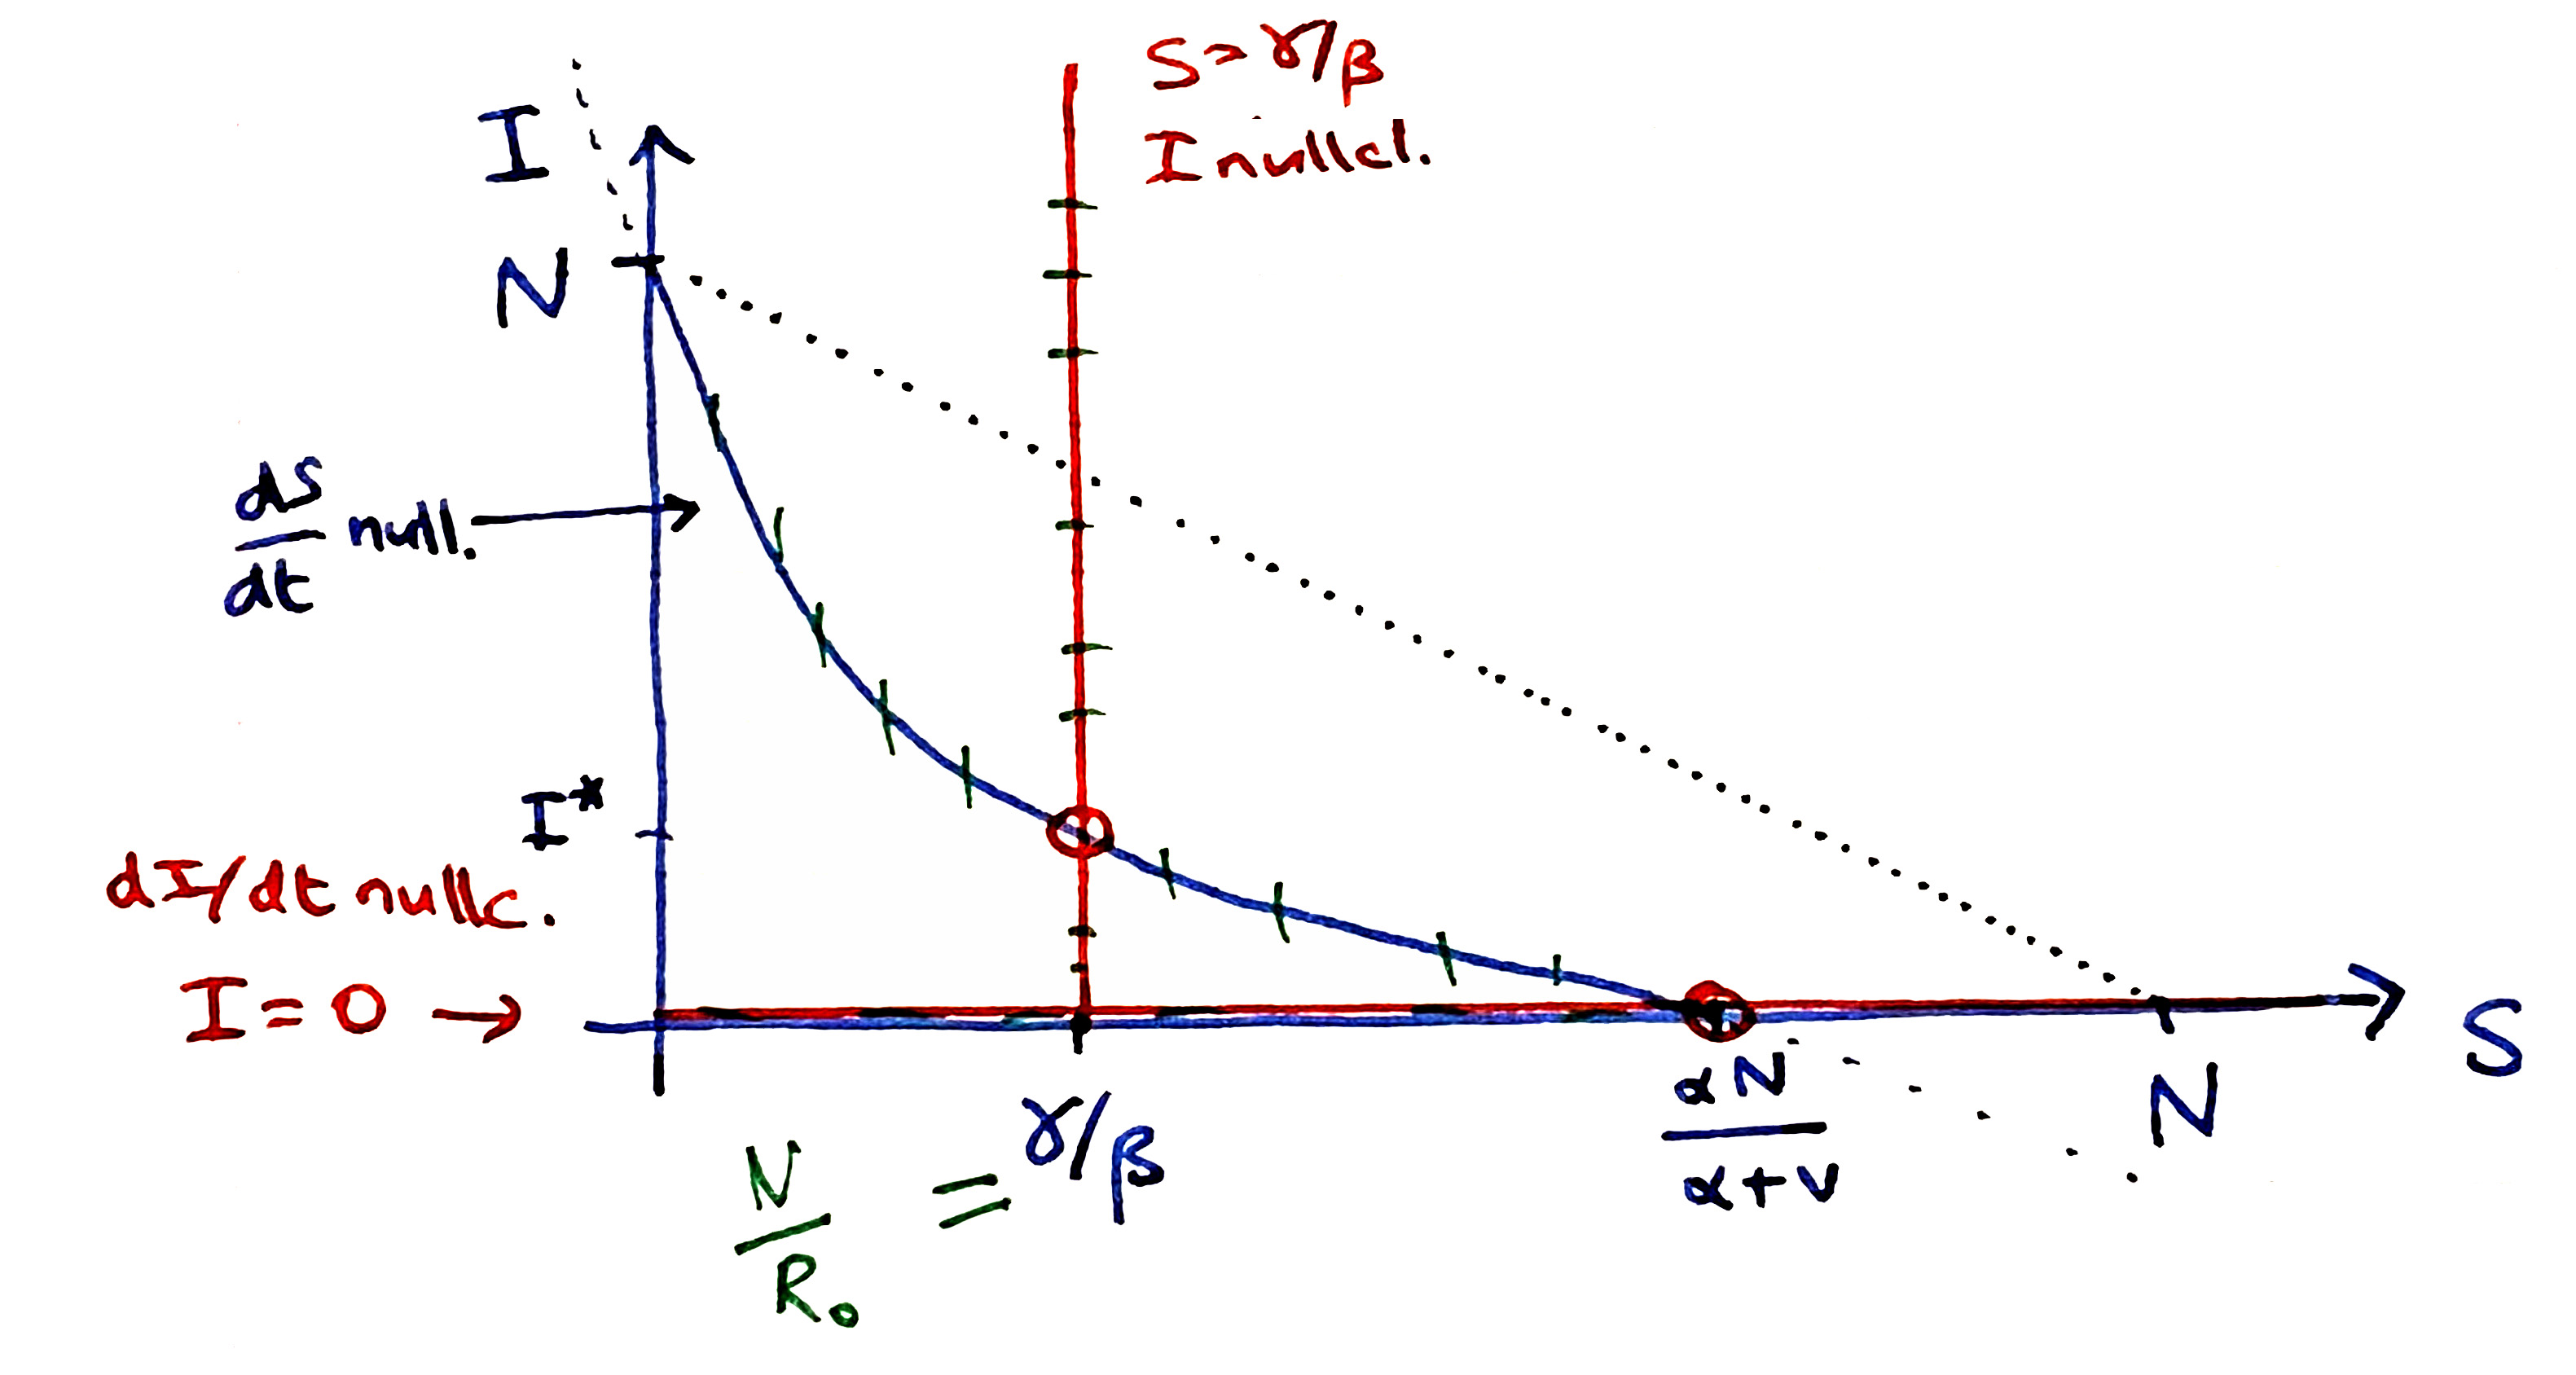
\includegraphics[width=0.7\textwidth]{images/sir-graph}
\end{center}
To draw the $I$ nullcline here, see that for small $S$, the equation for the nullcline looks like $-S$, and for large $S$, it looks like a constant.

There is no requirement in the question to put in trajectories, but if you wanted to, you could
\begin{enumerate}[label=(\roman*)]
	\item put in numbers to check a region, or
	\item try $(\varepsilon,\varepsilon)$,
\end{enumerate}
e.g.
\[\fd{S}{t}\sim\alpha N > 0, \qquad \fd{I}{t} \sim - \gamma \varepsilon < 0,\]

then use the fact that signs flip over the relevant nullclines.

\section{Travelling waves}
Travelling waves go from equilibrium to equilibrium. Which way? Think domino-o-oes.

For $x-ct$ you have a rightward travelling wave:
\begin{center}
stable \quad $\to$ \quad unstable

\textbackslash\textbackslash\textbackslash\textbackslash $\mid\mid\mid\mid\mid\mid\mid$
\end{center}

For $x+ct$ you have a leftward travelling wave:
\begin{center}
unstable \quad $\leftarrow$ \quad stable

$\mid\mid\mid\mid\mid\mid\mid$////
\end{center}

\end{document}
